\documentclass[12pt, a4paper]{article}

\usepackage{amsmath, amssymb, amsthm}
\usepackage{geometry}
\usepackage{graphicx}
\usepackage{hyperref}
\usepackage{enumitem}
\usepackage{booktabs}

\geometry{margin=2.5cm}

% Theorem environments
\theoremstyle{definition}
\newtheorem{definition}{Definition}[section]

\theoremstyle{plain}
\newtheorem{theorem}{Theorem}[section]

\theoremstyle{remark}
\newtheorem*{remark}{Remark}

\title{\textbf{The Tower of Hanoi}\\[0.4em]}
\author{0xHaru}
\date{\today}

\begin{document}

\maketitle

% ============================================================
\section{Preliminaries}
% ============================================================

\begin{definition}[Sequence]
A \emph{sequence} is a function from a subset of the set of integers
(usually either the set $\{0, 1, 2, \ldots\}$ or the set $\{1, 2, 3, \ldots\}$)
to a set $S$. We use the notation $a_n$ to denote the image of the integer $n$.
We call $a_n$ a \emph{term} of the sequence and we use the notation $\{a_n\}$ to refer to the sequence itself.
\end{definition}

\begin{definition}[Recurrence Relation]
A \emph{recurrence relation} for the sequence $\{a_n\}$ is an equation that
expresses $a_n$ in terms of one or more of the previous terms of the sequence,
namely, $a_0, a_1, \ldots, a_{n-1}$, for all integers $n$ with $n \ge n_0$,
where $n_0$ is a nonnegative integer. A sequence is called a \emph{solution}
of a recurrence relation if its terms satisfy the recurrence relation.
(A recurrence relation is said to \emph{recursively define} a sequence.)
\end{definition}

We say that we have solved a recurrence relation when we find an explicit
formula, called a \textbf{closed formula}, for the terms of the sequence.
Such a formula is only meaningful relative to a specific set of
\textbf{initial conditions}, which specify the terms that precede the first
one governed by the recurrence relation. Together, a recurrence relation and
its initial conditions uniquely determine the sequence, as one can prove by
\textbf{mathematical induction}.

% ============================================================
\section{The Tower of Hanoi}
% ============================================================

The Tower of Hanoi is a classic puzzle consisting of three pegs --- $P_1$,
$P_2$, $P_3$ --- and a stack of $n$ disks of decreasing size, all initially
placed on $P_1$. The goal is to move the entire stack to $P_3$, subject to two
rules: only one disk may be moved at a time, and no disk may ever be placed on
top of a smaller one.

\begin{figure}[h]
  \centering
  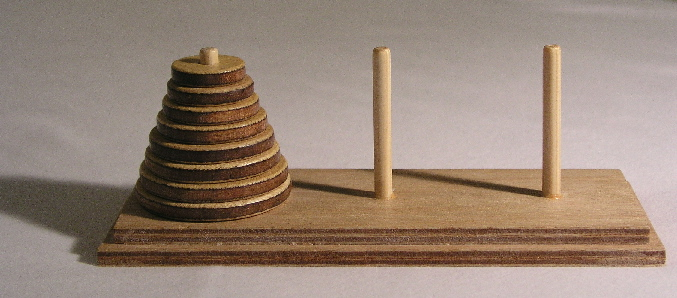
\includegraphics[width=0.55\textwidth]{tower_of_hanoi.jpg}
  \caption{A physical Tower of Hanoi puzzle with all disks stacked on $P_1$.}
\end{figure}

% ============================================================
\section{A Worked Example}
% ============================================================

We illustrate the puzzle with $n = 3$ disks. Label the disks $D_1$ (smallest),
$D_2$ (medium), and $D_3$ (largest), all initially stacked on $P_1$. The table
below shows the move sequence together with the resulting state of every peg
after each move, with disks listed from bottom to top. The puzzle is solved in
$2^3 - 1 = 7$ moves, confirming the formula we will derive in Section~5.

\begin{table}[h]
  \centering
  \renewcommand{\arraystretch}{1.3}
  \begin{tabular}{ccccc}
    \toprule
    \textbf{Move} & \textbf{Disk moved} & $P_1$ & $P_2$ & $P_3$ \\
    \midrule
    0 & (initial state) & $D_3,\, D_2,\, D_1$ & $-$ & $-$ \\
    1 & $D_1 \to P_3$   & $D_3,\, D_2$         & $-$ & $D_1$ \\
    2 & $D_2 \to P_2$   & $D_3$                & $D_2$ & $D_1$ \\
    3 & $D_1 \to P_2$   & $D_3$                & $D_2,\, D_1$ & $-$ \\
    4 & $D_3 \to P_3$   & $-$                  & $D_2,\, D_1$ & $D_3$ \\
    5 & $D_1 \to P_1$   & $D_1$                & $D_2$ & $D_3$ \\
    6 & $D_2 \to P_3$   & $D_1$                & $-$ & $D_3,\, D_2$ \\
    7 & $D_1 \to P_3$   & $-$                  & $-$ & $D_3,\, D_2,\, D_1$ \\
    \bottomrule
  \end{tabular}
  \caption{Solution of the Tower of Hanoi with $n = 3$ disks. Peg contents
  are listed from bottom to top; $-$ denotes an empty peg.}
\end{table}

% ============================================================
\section{Setting Up the Recurrence Relation}
% ============================================================

Let $H_n$ denote the number of moves needed to solve the Tower of Hanoi
problem with $n$ disks. We want to set up a recurrence relation for the
sequence $\{H_n\}$.

\bigskip

Begin with $n$ disks on $P_1$.
\begin{enumerate}[label=\textbf{Step \arabic*.}, leftmargin=*, itemsep=4pt]
  \item Transfer the top $n-1$ disks from $P_1$ to $P_2$ using $H_{n-1}$
        moves. The largest disk remains fixed on $P_1$ throughout.
  \item Use $1$ move to transfer the largest disk from $P_1$ to $P_3$.
  \item Transfer the $n-1$ disks from $P_2$ to $P_3$ using $H_{n-1}$
        additional moves, placing them on top of the largest disk and
        thus solving the puzzle.
\end{enumerate}

This reasoning shows that
\begin{equation}
  H_n = 2H_{n-1} + 1. \label{eq:rr}
\end{equation}

\noindent\textbf{Initial condition.}
Since a single disk can be transferred from $P_1$ to $P_3$ in exactly one
move, we have
\[
  H_1 = 1.
\]

\pagebreak

% ============================================================
\section{Solving the Recurrence Relation}
% ============================================================

We want to find a \emph{closed-form expression} for~\eqref{eq:rr}.
We use the \textbf{iterative approach}.

\subsection{Forward Iteration}

Applying the recurrence relation starting from the initial condition:
\begin{align*}
  H_1 &= 1,\\
  H_2 &= 2H_1 + 1 = 2(1) + 1 = 2 + 1,\\
  H_3 &= 2H_2 + 1 = 2(2+1) + 1 = 2^2 + 2 + 1,\\
  H_4 &= 2H_3 + 1 = 2(2^2+2+1) + 1 = 2^3 + 2^2 + 2 + 1.
\end{align*}

We begin to see the pattern:
\[
  H_k = 2^{k-1} + 2^{k-2} + \cdots + 2 + 1.
\]
Replacing $k$ with the general index $n$ gives the closed form:
\[
  H_n = 2^{n-1} + 2^{n-2} + \cdots + 2 + 1.
\]

\subsection{Backward Iteration}

We can reach the same conclusion by unrolling $H_n$ directly:
\begin{align*}
  H_n &= 2H_{n-1} + 1 \\
      &= 2\bigl(2H_{n-2}+1\bigr) + 1
       = 2^2 H_{n-2} + 2 + 1 \\
      &= 2^2\bigl(2H_{n-3}+1\bigr) + 2 + 1
       = 2^3 H_{n-3} + 2^2 + 2 + 1 \\
      &= 2^3\bigl(2H_{n-4}+1\bigr) + 2^2 + 2 + 1
       = 2^4 H_{n-4} + 2^3 + 2^2 + 2 + 1 \\
      &\;\vdots \\
      &= 2^{n-1} H_1 + 2^{n-2} + 2^{n-3} + \cdots + 2 + 1 \\
      &= 2^{n-1} + 2^{n-2} + \cdots + 2 + 1.
\end{align*}

The pattern after $k$ substitutions is always
\[
  H_n = 2^k H_{n-k} + 2^{k-1} + 2^{k-2} + \cdots + 2 + 1.
\]
We stop when the subscript reaches $1$, i.e.\
when $n - k = 1$, giving $k = n - 1$. Substituting:
\[
  H_n = 2^{n-1} H_1 + 2^{n-2} + \cdots + 2 + 1 = 2^{n-1} + 2^{n-2} + \cdots + 2 + 1,
\]
where the last equality uses $H_1 = 1$.

\medskip

We have reached the same conclusion by both approaches.
The expression on the right is a \emph{geometric series}.

\subsection{Closed Form via the Geometric Series Formula}

Recall that
\[
  a + ar + ar^2 + \cdots + ar^m
  = \sum_{k=0}^{m} ar^k
  = \begin{cases}
      \dfrac{a\,r^{m+1} - a}{r - 1} & \text{if } r \ne 1, \\[8pt]
      (m+1)\,a                       & \text{if } r = 1.
    \end{cases}
\]

In our case $a = 1$ and $r = 2$, so
\[
  H_n
  = \sum_{k=0}^{n-1} 2^k
  = \frac{2^{n-1+1} - 1}{2 - 1}
  = 2^n - 1.
\]

% ============================================================
\section{Verification by Induction}
% ============================================================

Now we want to show that $H_n = 2^n - 1$ is indeed a solution to the
recurrence relation $H_n = 2H_{n-1} + 1$ with initial condition $H_1 = 1$.
We do so by induction on $n$.

\begin{theorem}
  The sequence defined by
  \[
    H_n = 2H_{n-1} + 1, \quad H_1 = 1,
  \]
  has the closed-form solution $H_n = 2^n - 1$ for all integers $n \ge 1$.
\end{theorem}

\begin{proof}
We proceed by induction on $n$.

\medskip
\noindent\textbf{Base case} ($n = 1$).
\[
  2^1 - 1 = 1 = H_1.
\]

\medskip
\noindent\textbf{Inductive step.}
Assume the formula holds for some integer $n \ge 1$, i.e.,
\[
  H_n = 2^n - 1 \tag{IH}.
\]
We wish to show that $H_{n+1} = 2^{n+1} - 1$.

By the recurrence relation~\eqref{eq:rr},
\[
  H_{n+1} = 2H_n + 1.
\]
Substituting the inductive hypothesis (IH):
\[
  H_{n+1}
  = 2\!\left(2^n - 1\right) + 1
  = 2^{n+1} - 2 + 1
  = 2^{n+1} - 1,
\]
which is precisely the formula evaluated at $n+1$.

\medskip
By the principle of mathematical induction, $H_n = 2^n - 1$ holds for
all integers $n \ge 1$.
\end{proof}

\bigskip

\begin{remark}
The Tower of Hanoi puzzle with $n$ disks requires exactly $2^n - 1$ moves ---
an exponential number of moves in the size of the input.
\end{remark}

\end{document}
